\section{Simboličko izračunavanje}
\label{sec:Symbolics}

Tokom procesa pronalaženja grešaka u radu softvera koriste se ručno pisani testovi i pregledi koda od strane drugih programera, i ove mere provere koda mogu verifikovati da softver, ili deo softvera, funkcioniše na različitim nivoima komplikovane arhitekture velikih projekata. Uprkos svim ovim merama, greške su i dalje nezaobilazne - jedan test može proveriti ponašanje koda za samo jedan ulaz. S obzirom da je nemoguće testirati sve moguće ulaze zbog njihovog ogromnog broja (ukoliko posmatramo samo funkciju jedne promenljive koja prima 32-bitni ceo broj, broj mogućih ulaza je $2^{32}$) nadamo se da testovi dobro \emph{generalizuju} - da pokrivaju opšte ali i neke specijalne ulaze. To se postiže uočavanjem da se vrednosti ulaza mogu razvrstati u klase po tome kakav izlaz uzrokuju. Ukoliko imamo funkciju koja treba da podeli dva broja, te klase mogu biti celi brojevi, realni brojevi, neke specijalne vrednosti specifične za to šta se testira (u ovom slučaju, $0$), kao i granice za tip podataka iz čijeg domena argumenti mogu uzeti vrednost. Čak i ovakav pristup, iako drastično smanjuje broj testova i eliminiše redundantne testove, i dalje zahteva relativno veliki broj testova u slučaju većih projekata i stoga je teško pronaći sve greške, pogotovo u slučajevima koji se retko dešavaju i zavise recimo od stanja drugih komponenti ili pak nekih nedeterminističkih ponašanja. U komplikovanim projektima je teško pokriti čitav izvorni kod testovima (engl. \emph{code coverage}) - iako pokrivenost koda od 100\% i dalje ne znači da taj kod ispravno radi.

\emph{Statička analiza koda} predstavlja analizu izvornog koda bez pokretanja istog. Ideja je baš ispitivanje svih mogućih stanja u kojima se može naći program i testiranje svih mogućih ulaza u jedinicu koja se testira. U praksi se nailazi na puno problema - osnovni je razlika simboličke i programerske apstrakcije. 

Simboličko izvršavanje \cite{SymbolicExecution} predstavlja sredinu između klasične verifikacije putem pisanja testova i statičke analize koda. Prilikom simboličkog izvršavanja, umesto stvarnih vrednosti ulaza koje se koriste u testovima, koriste se \emph{simboličke promenljive}. Simbolička promenljiva nije vezana za specifičnu vrednost i analiza se dalje vrši samo nad njom - samim tim se istovremeno mogu testirati višestruke klase sličnih ulaza. 

Primer simboličkog izvršavanja će biti opisan na isečku C sa slike \ref{fig:SymbolicExecCode}. Pretpostavimo da imamo deklarisanje promenljive \texttt{a}, \texttt{b} i \texttt{c} i da se neke operacije izvršavaju nad njima, reprezentovano komentarom. U nekom trenutku se vrednosti tih promenljivih koriste kao uslovi od kojih zavisi prolaznost testa u poslednjoj liniji. Dodelimo svakoj promenljivoj simboličku vrednost - \texttt{a = }$\alpha$, \texttt{b = }$\beta$, \texttt{c = }$\gamma$. Možemo izgraditi stablo izvršavanja i uslove koji moraju da važe nad simboličkim vrednostima $\alpha$, $\beta$ i $\gamma$ kako bi test u poslednjoj liniji prošao.

\begin{figure}[h!]
    \begin{lstlisting}[language={}]
    int a, b, c;

    // ...

    int x = 0; int y = 0; int z = 0;
    if (a)      
        x = -2;
    if (b < 5)  {
        if (!a && c)    
            y = 1;
        z = 2;
    }

    assert(x + y + z != 3);
    \end{lstlisting}
    \caption{Isečak C koda dat kao primer nad kojim će se prikazati simboličko izvršavanje.}
    \label{fig:SymbolicExecCode}
\end{figure}

Ukoliko put izvršavanja programa zavisi od simboličke promenljive, kao što je to slučaj za izvorni kod sa slike \ref{fig:SymbolicExecCode}, simbolička promenljiva se konceptualno "grana" i analiza se nastavlja za oba slučaja posebno. Tako se dobija drvo izvršavanja, gde svaki put odgovara mnogim individualnim testovima koji bi uzrokovali prolazak izvršavanja tim putem. Vrednosti promenljivih u tim testovima moraju zadovoljiti uslove na kraju svakog puta - tzv. \emph{uslove puta} (engl. \emph{path conditions}). Odgovarajuće stablo izvršavanja za izvorni kod sa slike \ref{fig:SymbolicExecCode} sa definisanim simboličkim vrednostima $\alpha$, $\beta$ i $\gamma$ se može videti na slici \ref{fig:SymbolicExecTree}. Svaka naredba dodele je uokvirena pravougaonikom dok je uslov uokviren elipsom. Boje grana odgovaraju istinitosnoj vrednosti uslova iz poslednje linije koda u tom trenutku. Na kraju svake grane se nalazi uslov puta za tu granu koje u nekim slučajevima može jedinstveno odrediti vrednost simboličke promenljive koja dovodi do prolaska tim putem ili u opštem slučaju generisati test primer koji dovodi do prolaska tim putem. Dakle, ukoliko je stablo simboličkog izvršavanja poznato, moguće je trivijalno generisati kontra-primere koji dokazuju da program ne radi kao što je očekivano.

\begin{figure}[h!]
    \centering
    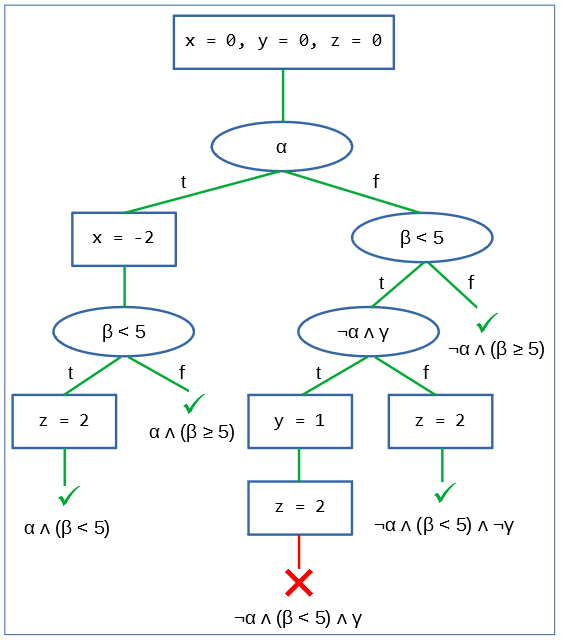
\includegraphics[scale=0.8]{images/sym_tree.png}
    \caption{Drvo simboličkog izvršavanja na kom su prikazane sve putanje koje se razmatraj. Na kraju svake grane je napisan uslov koji mora da važi da bi se došlo do tog lista u drvetu.}
    \label{fig:SymbolicExecTree}
\end{figure}

Simboličko izvršavanje, iako konceptualno moćno, ima par problema:
\begin{itemize}
    \item \emph{eksplozija putanja} - Broj puteva izvršavanja eksponencijalno zavisi od broja uslovnih grananja u kodu. Ukoliko imamo 3 naredbe grananja, broj puteva izvršavanja je $2^3=8$. Štaviše, petlje su još komplikovanije, jer ukoliko imamo u petlji uslov koji zavisi od simboličke vrednosti koja uzima vrednosti iz opsega 32-bitnog celog broja, broj puteva kroz petlju je u tom slučaju $2^31$, a u komplikovanijim slučajevima i beskonačan. Slično važi i za rekuriju.
    \item \emph{ograničenja rešavača} - U nekim slučajevima je moguće osloniti se na \emph{SMT rešavače} \cite{SMT} za nalaženje kontra-primera.
    \item \emph{modelovanje podataka} (engl. \emph{heap modelling}) - Kreiranje simboličkih struktura podataka i pokazivača nije jednostavna.
    \item \emph{modelovanje okruženja} (engl. \emph{environment modelling}) - Nije uvek jednostavno adaptirati mehanizam da radi sa čestim potrebama prilikom dizajna softvera - eksterne biblioteke i sistemski pozivi, specifičnosti sistema i okruženja.
\end{itemize}

Postoji dosta alata i biblioteka koje pružaju simboličko izračunavanje - jedan od najpoznatijih alata za simboličko izračunavanje je \emph{KLEE} \cite{KLEE}, izgrađen nad \emph{LLVM} infrastruktorom \cite{LLVM} i dizajniran za analizu koda pisanog u programskom jeziku C. U nastavku će simboličko izvršavanje biti korišćeno za detekciju razlika u vrednostima promenljivih iz dva AST-a kroz biblioteke za rad sa simboličkim vrednostima u programskom jeziku C\#.
